\documentclass[a4paper,12pt]{report}

\usepackage{cmap}
\usepackage[T2A]{fontenc}
\usepackage[utf8]{inputenc}
\usepackage[russian]{babel}
\usepackage{amsmath,amsfonts,amssymb}
\usepackage{graphicx}
\usepackage{sidecap}
\usepackage{wrapfig}
\usepackage{indentfirst}

\begin{document} 

\begin{titlepage} 

\begin{center} 

\large Федеральное государственное автономное образовательное учреждение высшего образования «Санкт-Петербургский государственный электротехнический университет «ЛЭТИ» им. В.И. Ульянова (Ленина)»\\
кафедра Вычислительной техники\\[5cm] 

\huge ОТЧЕТ\\ по лабораторной работе № 3\\[0.5cm] 
\large <<Применение функций>>\\[3.7cm]

\begin{minipage}{1\textwidth}
    \begin{flushleft}
        \emph{Автор:} Стукен В.А.\\
        \emph{Группа:} 2307\\
        \emph{Факультет:} ФКТИ\\
        \emph{Преподаватель:} Аббас Саддам Ахмед\\
    \end{flushleft}
\end{minipage}

\vfill

Санкт-Петербург, 2022\\
{\large \LaTeX}

\end{center}
\thispagestyle{empty}
\end{titlepage}

\section*{Задание(вариант 3)}
Ввести построчно элементы двумерного массива чисел. Количество столбцов задается. Количество строк в массиве, но не менее одной, равно максимальному по модулю элементу начальной (нулевой) строки. Из столбцов исходного массива, которые образуют неубывающую последовательность чисел, сформировать строки результирующего массива. Вывести сформированный массив. Ввод строки массива и формирование строки результирующего массива оформить в виде функций.

\section*{Постановка задачи и описание решения}
\par

Сначала прогамма считывает количество столбцов массива(cols), далее инициализируем массив $a$ целых чисел длиной равной количеству столбцов. 
В функцию $scan\_row$ передаем этот массив и количество столбцов. 
Функция $scan\_row$ заполняет массив $a$.
По условию задачи количество строк в матрице равно по модулю максимальному элементу массива $a$.
Теперь задаем двумерный массив $arr$ размерами $rows \cdot cols$, где $rows$ - максимальный по модулю элемент $a$.
Далее с помощью функции $scan\_row$ задаем каждую строку массива $arr$.
Инициализируем массив $out\_arr$, который мы должны получить в результате работы программы, размерами $cols \cdot rows$
Далее задаем массив $curr\_col$ размером $rows$, в котором будет храниться текущий столбец массива. Этот массив передаем в функцию $form\_row$,
которая возвращает 1, если последовательность не убывающая и 0 - если убывающая, а также заполняет строки массива $out\_arr$
соответсвенными элементами столбцов массива $arr$

Далее программа выводит полученный массив.


\section*{Описание переменных}
\begin{centering}
\resizebox{14cm}{!}{
    \begin{tabular}{|l|l|l|l|}
        \hline
        \textbf{№} & \textbf{Имя переменной} & \textbf{Тип} & \textbf{Назначение}\\
        \hline
        1 & cols          &int& Количество столбцов исходного массива\\ 
        \hline
        2 &   mx            & int  & Максимальный элемент первой строки массива\\ 
        \hline
        3 &  a          &  int[] & Первая строка массива \\
        \hline
        4 & rows        & int & Количество строк в исходном массиве\\ 
        \hline
        5 & arr             & int[][] & Исходный массив \\
        \hline
        6  &   out\_arr      & &\\
        \hline
    \end{tabular}
}
\end{centering}

\section*{Контрольные примеры}

\begin{centering}
\resizebox{12cm}{!}{
    \begin{tabular}{|l|l|}
        \hline
          \textbf{Входные данные} & \textbf{Выходные данные}\\
        \hline
            3        & 1 0 1 0\\ 
            3        & 1 0 0 1\\ 
            1 0 1    & 0 1 1 0\\
            1 0 0    &        \\
            0 1 1    &        \\
        \hline
            5        & 1 0 1 0 0\\ 
            4        & 1 0 0 1 0\\ 
            1 0 1 0  & 0 1 1 1 1\\
            1 0 0 1  & 1 0 1 1 1\\
            0 1 1 1  & 0 0 0 0 0\\
            1 0 1 1  &          \\
            0 0 0 0  &          \\
        \hline
    \end{tabular}
}
\end{centering}
\newpage

\section*{Примеры использования программы}
    \begin{figure}[h]
        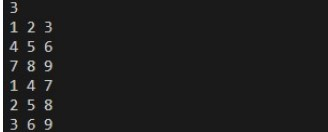
\includegraphics[width=0.5\textwidth]{ex1.jpg}
    \caption{Входные данные 1}
    \label{ris:image1}
            
        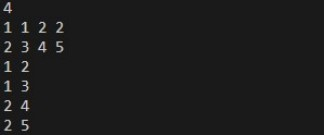
\includegraphics[width=0.5\textwidth]{ex2.jpg}
    \caption{Входные данные 2}
    \label{ris:image2}
    
    \end{figure}

\section*{Вывод}
В результате выполнения лабораторной работы изучили работу с двумерными массивами в Си и научились обрабатывать их элементы.

\end{document}